\documentclass[notheorems,aspectratio=169]{beamer}

\author{Владислав Шаршуков}
\date{\today}
\title{Робастность дискретных систем}

%% \usetheme{Warsaw}
\usetheme{default}
\usefonttheme{serif}

\usepackage[utf8]{inputenc}
\usepackage[T2A]{fontenc}
\usepackage[russian]{babel}
\usepackage{graphicx}
\usepackage{longtable}
\usepackage{wrapfig}
\usepackage{rotating}
\usepackage[normalem]{ulem}
\usepackage[makeroom]{cancel}
\usepackage{amsmath}
\usepackage{amssymb}
\usepackage{capt-of}
\usepackage{hyperref}

\usepackage[backend=biber]{biblatex}
%% \usepackage[backend=biber,citestyle=authortitle]{biblatex}

\graphicspath{ {./Images/} }

\addbibresource{DiscreteRobustness.bib}

\theoremstyle{definition}
\newtheorem{theorem}{Теорема}
\newtheorem{definition}{Определение}
\newtheorem{remark}{Замечание}
\newtheorem{proposition}{Утверждение}
\newtheorem{lemma}[theorem]{Лемма}
\newtheorem{corollary}[theorem]{Следствие}

%% \hypersetup{
%%   pdfauthor={Владислав Шаршуков},
%%   pdftitle={Робастность дискретных систем},
%%   pdfkeywords={},
%%   pdfsubject={},
%%   pdflang={Russian}}

\newcommand{\highlight}[1]{{\color{red} #1}}
\newcommand{\abs}[1]{\left| #1 \right|}
\newcommand{\paren}[1]{\left( #1 \right)}
\renewcommand{\emph}[1]{\uline{#1}}
\renewcommand{\Re}{\operatorname{Re}}
\renewcommand{\Im}{\operatorname{Im}}

\setbeamertemplate{section in toc}[sections numbered]
\setbeamertemplate{footline}{}
\setbeamertemplate{headline}{}
\setbeamertemplate{navigation symbols}{}

%% ================================== %%
\begin{document}

\begin{frame}
  \titlepage
\end{frame}

\begin{frame}{Содержание}
  \tableofcontents
\end{frame}

\section{Дискретные системы. Введение, устойчивость}
%% \begin{frame}{Дискретные системы: применение}
%% \end{frame}

\begin{frame}{Разностное уравнение. $z$-преобразование}
  Разностное уравнение (в обратных разностях):
  \begin{equation*}
    \nabla^N y(n) + \alpha_1 \nabla^{N-1} y(n) + \cdots + \alpha_N y(n) = 
    \beta_0 \nabla^M x(n) + \beta_1 \nabla^{M-1} x(n) + \cdots + \beta_M x(n).
  \end{equation*}

  $z$-преобразование:
  \begin{equation*}
    Z\left\{ f(n) \right\} = F(z) = \sum_{n=0}^\infty f(n) z^{-n}.
  \end{equation*}

  Таблицу $z$-преобразований можно найти в \cite[с.~255]{Kargu1974}.
\end{frame}

\begin{frame}{Передаточная функция. Характеристический полином}
  \begin{definition}
    \textit{Передаточной функцией} разностной системы называют отношение
    $z$-преобразования выходной последовательности $y(n)$ к $z$-преобразованию
    входной последовательности $x(n)$ при нулевых начальных условиях:
    \begin{equation*}
      \Phi(z) = \frac{Z\left\{ y(n) \right\}}{Z\left\{ x(n)\right\}} = \frac{Y(z)}{X(z)}.
    \end{equation*}
  \end{definition}

  \begin{definition}
    Знаменатель передаточной функции $X(z)$ называют \textit{характеристическим полиномом} разностного уравнения.
  \end{definition}
\end{frame}

\begin{frame}{Пример}
  Разностное уравнение:
  \begin{equation*}
    y(n) + (\alpha - 1) y(n - 1) = \alpha x(n), \quad 0 < \alpha < 1.
  \end{equation*}
  Применим $z$-преобразование при нулевых начальных данных ($y(-1) = 0$):
  \begin{equation*}
    Y(z) + (\alpha - 1) z^{-1} Y(z) = \alpha X(z).
  \end{equation*}
  Передаточная функция:
  \begin{equation*}
    \Phi(z) = \frac{Y(z)}{X(z)} = \frac{\alpha}{1 + (\alpha - 1) z^{-1}} = \frac{\alpha z}{z + (\alpha - 1)}.
  \end{equation*}

  Характеристический полином: $z + (\alpha - 1)$.
\end{frame}

\begin{frame}{Область устойчивости дискретной системы}
  Характеристический полином системы:
  \begin{equation*}
    a(z) = a_0 z^m + a_1 z^{m-1} + \cdots + a_m = a_0 \prod_{i=1}^m (z - z_i).
  \end{equation*}

  \begin{proposition}[{\cite[с.~259]{Kargu1974}}]
    Для устойчивости дискретной системы необходимо, чтобы корни её характеристического полинома
    $a(z)$ лежали внутри единичной окружности:
    \begin{equation*}
      \abs{z_i} < 1 \quad \forall i=\overline{1,m}.
    \end{equation*}
  \end{proposition}
\end{frame}

\begin{frame}{Скрытая неустойчивость}
  \begin{remark}
    Условие $\abs{z_i} < 1, \; \forall i=\overline{1,m}$ гарантирует устойчивость только в дискретные моменты времени,
    поэтому возможны случаи ``скрытой'' неустойчивости, когда $y(n)$ затухает, а $y(t)$ не затухает или расходится:
    \begin{center}
      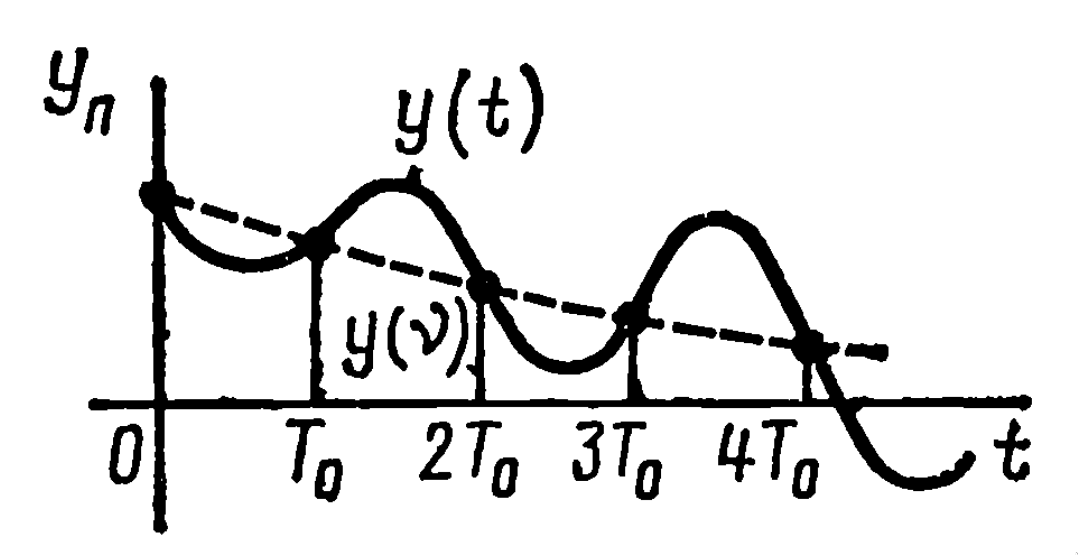
\includegraphics[width=8cm]{HiddenInstability}
    \end{center}
  \end{remark}
\end{frame}

\begin{frame}{Билинейное преобразование}
  \begin{proposition}[{\cite[с.~1214]{KrausAndersonMansour1988}}]
    Если все корни полинома $f(z)$ лежат в единичной окружности, то все корни полинома
    \begin{equation*}
      g(s) = (s - 1)^n f\paren{\frac{s+1}{s-1}}
    \end{equation*}
    лежат в левой полуплоскости $\Re{s} < 0$.
  \end{proposition}
\end{frame}

\section{Теоремы Харитонова. Неприменимость в дискретном случае}

\begin{frame}{Интервальный полином}
  \begin{definition}
    \textit{Интервальным полиномом} называется семейство полиномов
    \begin{equation}\label{def:interval-polynomial}
      F(s) = \sum_{k=0}^n a_k s^k,
      \quad a_k \in [\underline{a}_k, \overline{a}_k],
      \quad \underline{a}_k \leqslant \overline{a}_k
      \quad \forall k=\overline{0,n}
    \end{equation}
  \end{definition}

  \begin{definition}
    \textit{Угловыми полиномами} называются полиномы вида
    \eqref{def:interval-polynomial}, где либо \(a_k = \underline{a}_k\), либо
    \(a_k = \overline{a}_k\) для всех \(k=\overline{1,n}\).
  \end{definition}
\end{frame}

\begin{frame}{Теоремы Харитонова}
  \begin{theorem}[Харитонова, слабая]
    Необходимым и достаточным условием робастной устойчивости интервального
    полинома является гурвицевость всех его угловых полиномов.
  \end{theorem}

  \begin{theorem}[Харитонова, сильная]
    Необходимым и достаточным условием робастной устойчивости интервального
    полинома является гурвицевость лишь четырёх полиномов:

    \begin{equation}
      \begin{aligned}
        F_1(s) &= \underline{a}_0 + \overline{a}_1 s + \overline{a}_2 s^2 +
        \underline{a}_3 s^3 + \underline{a}_4 s^4 + \dots \\
        F_2(s) &= \underline{a}_0 + \underline{a}_1 s + \overline{a}_2 s^2 +
        \overline{a}_3 s^3 + \underline{a}_4 s^4 + \dots \\
        F_3(s) &= \overline{a}_0 + \underline{a}_1 s + \underline{a}_2 s^2 +
        \overline{a}_3 s^3 + \overline{a}_4 s^4 + \dots \\
        F_4(s) &= \overline{a}_0 + \overline{a}_1 s + \underline{a}_2 s^2 +
        \underline{a}_3 s^3 + \overline{a}_4 s^4 + \dots
      \end{aligned}
    \end{equation}
  \end{theorem}
\end{frame}

\begin{frame}{Контрпример для дискретного случая}
  Рассмотрим многочлен
  \begin{equation}
    g(b_1, z) = z^4 + b_1z^3 + \frac{3}{2} z^2 - \frac{1}{3}, \quad b_1 \in \left[\frac{-17}{8}, \frac{17}{8}\right].
  \end{equation}

  Полиномы $g(-17/8, z)$ и $g(17/8, z)$ являются полиномами Шура, а $g(0, z)$ -- нет.
\end{frame}

\begin{frame}{Трудности применения билинейного преобразования}
  Матрица билинейного преобразования неортогональна, следовательно, преобразование
  не сохраняет \textit{прямоугольность} области изменения коэффициентов характеристического полинома $f(z)$ дискретной системы.
\end{frame}

\begin{frame}{Пример}
  Характеристический полином: $f(z) = az^2, \quad a \in [1, 2]$.

  Применяем билинейное преобразование:
  \begin{equation*}
    \begin{aligned}
      g(s) &= (s-1)^n f\paren{\frac{s+1}{s-1}} \\
      &= \cancel{(s - 1)^2} \cdot a \frac{(s + 1)^2}{\cancel{(s - 1)^2}} \\
      &= as^2 + 2as + a.
    \end{aligned}
  \end{equation*}

  Область изменения коэффициентов многочлена $g(s)$ непрямоугольна, поэтому теорема Харитонова неприменима.
\end{frame}

\section{Дискретный аналог: слабая теорема Харитонова}

\begin{frame}{Аналог, вариант, эквивалент \cite{JuryMansour1985}}
  \begin{itemize}
  \item \textit{Дискретный \emph{аналог} критерия} --- критерий в дискретном случае по \emph{форме}
    совпадает с критерием в непрерывном случае
  \item \textit{Дискретный \emph{вариант} критерия} --- критерий в дискретном случае по \emph{сути}
    совпадает с критерием в непрерывном случае
  \item \textit{Дискретный \emph{эквивалент} критерия} --- критерий в дискретном случае по \emph{форме} и \emph{сути}
    совпадает с критерием в непрерывном случае

  \end{itemize}
\end{frame}

\begin{frame}{Вспомогательные определения}
  Рассмотрим полином
  \begin{equation*}
    D(z) = d_0 + d_1 z + \cdots + d_n z^n.
  \end{equation*}

  Введём обозначение:
  \begin{equation*}
    D^*(z) = z^n D(z^{-1}) = d_0 z^n + d_1 z^{n-1} + \cdots + d_n.
  \end{equation*}

  \begin{definition}
    Полином $S(z)$ называется \textit{симметричным}, если $S^*(z) = S(z)$.
  \end{definition}

  \begin{definition}
    Полином $A(z)$ называется \textit{антисимметричным}, если $A^*(z) = -A(z)$.
  \end{definition}
\end{frame}

\begin{frame}{Вспомогательные определения}
  \begin{proposition}[{\cite{Bistritz1984}}]
    Любой многочлен $D_k(z)$ степени $k$ с вещественными коэффициентами
    может быть записан как сумма симметричного и антисимметричного многочленов:

    \begin{equation*}
      D_k(z) = S_k(z) + A_k(z),
    \end{equation*}
    где
    \begin{equation*}
      \begin{aligned}
        S_k(z) &= \frac{1}{2} \left[ D_k(z) + D_k^*(z) \right] \\
        A_k(z) &= \frac{1}{2} \left[ D_k(z) - D_k^*(z) \right]
      \end{aligned}
    \end{equation*}
  \end{proposition}

  \begin{proof}
    Утверждение проверяется непосредственной подстановкой.
  \end{proof}
\end{frame}

\begin{frame}{Демонстрация подхода}
  Рассмотрим многочлен
  \begin{equation*}
    F(z) = \sum_{i=0}^n a_{i} z^i = a_0 \prod_{i=0}^n \paren{z - z_i}, \quad a_i \in \mathbb{R}.
  \end{equation*}

  Определим его симметричную и антисимметричную части:
  \begin{equation*}
    F(z) = F_1(z) + F_2(z),
  \end{equation*}
  где
  \begin{equation*}
    \begin{aligned}
      F_1(z) &= \frac{1}{2} \left[ F(z) + F^*(z) \right] \\
      F_2(z) &= \frac{1}{2} \left[ F(z) - F^*(z) \right] \\
    \end{aligned}
  \end{equation*}
\end{frame}

\begin{frame}{Демонстрация подхода: теорема}
  \begin{theorem}[{\cite{Gnanasekaran1981,Schussler1976}}]
    Полином $F(z)$ устойчив тогда и только тогда, когда выполняются условия:
    \begin{enumerate}
    \item Корни полиномов $F_1(z)$ и $F_2(z)$ лежат на единичной окружности;
    \item Они простые;
    \item Они перемежаются;
    \item $\abs{\dfrac{a_0}{a_n}} < 1$.
    \end{enumerate}
  \end{theorem}

  %%   \begin{remark}
  %%     Условия 1-3 эквивалентны 
  %%   \end{remark}
\end{frame}

\begin{frame}{Доказательство: необходимость}
  \begin{enumerate}
  \item Если корни $F(z)$ лежат внутри единичной окружности, то корни $F^*(z)$ будут лежать снаружи. Сравнивая множители
    $(z - z_i)$ в $F(z)$ и $z(z^{-1} - z_i)$ в $F^*(z)$, найдём, что
    \begin{equation}\label{eq:relations_1}
      \begin{cases}
        \abs{F(z)} < \abs{F^*(z)}, & \abs{z} < 1 \\
        \abs{F(z)} = \abs{F^*(z)}, & \abs{z} = 1 \\
        \abs{F(z)} > \abs{F^*(z)}, & \abs{z} > 1.
      \end{cases}
    \end{equation}
    Введём обозначение
    \begin{equation*}
      Q(z) = \frac{F(z)}{F^*(z)};
    \end{equation*}
    тогда условия перепишутся в виде
    \begin{equation}\label{eq:relations_2}
      \begin{cases}
        \abs{Q(z)} < 1, & \abs{z} < 1, \\
        \abs{Q(z)} = 1, & \abs{z} = 1, \\
        \abs{Q(z)} > 1, & \abs{z} > 1.
      \end{cases}
    \end{equation}
  \end{enumerate}
\end{frame}

\begin{frame}{Доказательство: необходимость}
  \begin{enumerate}
    \setcounter{enumi}{1}
  \item Введём обозначение:
    \begin{equation*}
      \Phi(z) = \frac{F(z) + F^*(z)}{F(z) - F^*(z)} = \frac{F_1(z)}{F_2(z)} = \frac{Q(z) + 1}{Q(z) - 1}.
    \end{equation*}
    Тогда из условий \eqref{eq:relations_2} следует, что
    \begin{equation}\label{eq:relations_3}
      \Re \left\{ \Phi(z) \right\} = \frac{\abs{Q(z)}^2 - 1}{\abs{Q(z) - 1}^2}
      \begin{cases}
        < 0, & \abs{z} < 1, \\
        = 0, & \abs{z} = 1, \\
        > 0, & \abs{z} > 1.
      \end{cases}
    \end{equation}
  \end{enumerate}
\end{frame}

\begin{frame}{Доказательство: необходимость}
  \begin{enumerate}
    \setcounter{enumi}{2}
  \item Если $z = z_k = \abs{z_k} e^{j \psi_k}$ --- полюс порядка $m$ функции $\Phi(z)$, то для всех достаточно близких $z$
    \begin{equation*}
      \Phi(z) \approx \frac{R_{km}}{(z - z_k)^m} = \frac{\abs{R_{km}}}{\rho^m} e^{j (-m\alpha + \beta_k)},
    \end{equation*}
    где $R_{km} = \abs{R_{km}} e^{j \beta_k}$, $z - z_k = \rho e^{j\alpha}$, $\rho$ достаточно мал и $0 \leqslant \alpha \leqslant 2\pi$.
    Отсюда
    \begin{equation*}
      \Re \left\{ \Phi(z) \right\} \approx \frac{\abs{R_{km}}}{\rho^m} \cos\paren{m \alpha - \beta_k}.
    \end{equation*}
    Знак $\Re \left\{ \Phi(z) \right\}$ определяется знаком $\cos\paren{m \alpha - \beta_k}$, изменяющимся $2m$ раз
    при изменении $\alpha$ от $0$ до $2\pi$.
  \end{enumerate}
\end{frame}

\begin{frame}{Доказательство: необходимость}
  \begin{center}
    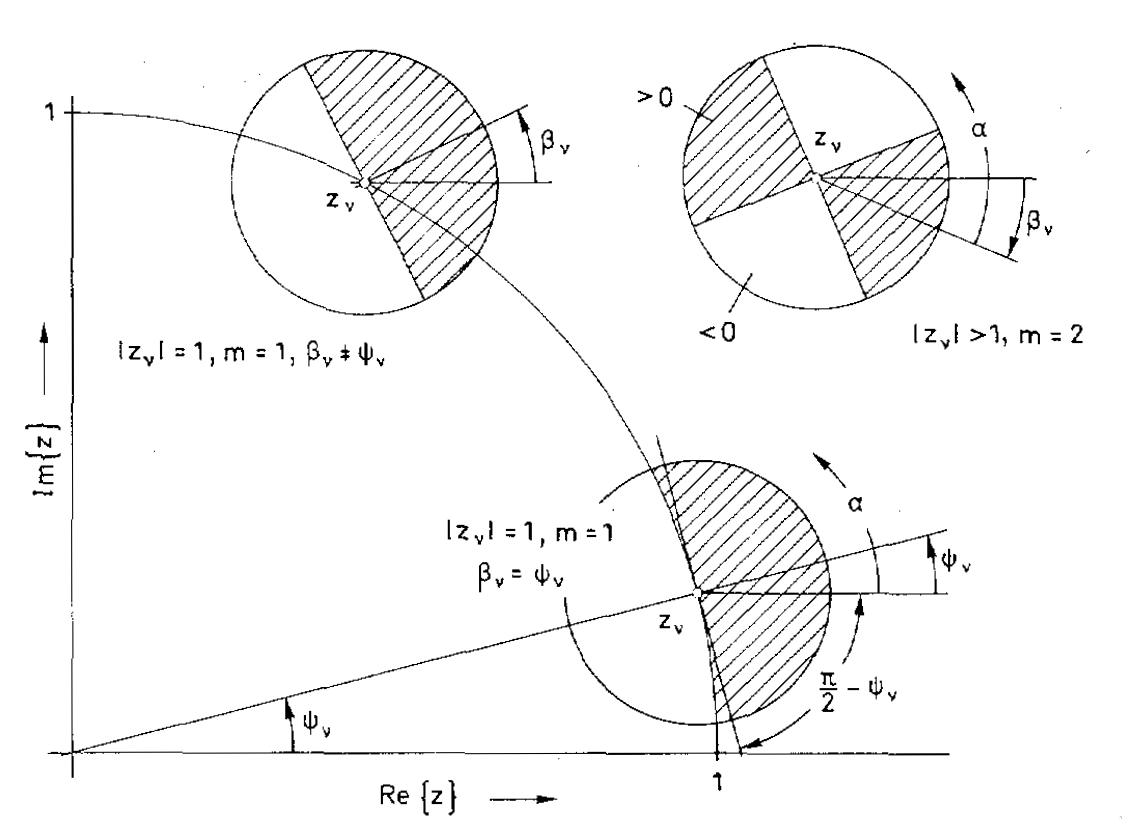
\includegraphics[width=6cm]{Poles}
  \end{center}

  Из \eqref{eq:relations_3} следует, что знак $\Re \left\{ \Phi(z) \right\}$
  может измениться только на пересечении с единичной окружностью, что влечёт за собой
  условия
  \begin{equation}
    \abs{z_k} = 1, \quad m = 1,
  \end{equation}
  т.е. полюсы функции $\Phi(z)$ простые, лежащие на единичной окружности.
\end{frame}

\begin{frame}{Доказательство: необходимость}
  Следовательно, для достаточно малых $\rho$,
  \begin{equation*}
    \Re \left\{\Phi(z)\right\} \approx \frac{\abs{R_{k}}}{\rho} \cos\paren{\alpha - \beta_k},
  \end{equation*}
  причём
  \begin{equation*}
    \Re \left\{ \Phi(z) \right\} > 0 \quad \mbox{ для } -\frac{\pi}{2} < \paren{\alpha - \beta_k} < \frac{\pi}{2}.
  \end{equation*}
  Знак $\Re \left\{ \Phi(z) \right\}$ изменяется только на пересечении с единичной окружностью, поэтому
  \begin{equation*}
    \Re \left\{ \Phi(z) \right\} > 0 \quad \mbox{ для } -\paren{\frac{\pi}{2} - \psi_k} < \alpha < \frac{\pi}{2} + \psi_k.
  \end{equation*}
  Отсюда $\beta_k = \psi_k$.

  Аналогичный результат достигается для $\dfrac{1}{\Phi(z)}$.
\end{frame}

\begin{frame}{Доказательство: необходимость}
  \begin{enumerate}
    \setcounter{enumi}{3}
  \item Покажем перемежаемость корней $F_1(z)$ и $F_2(z)$.

    В соответствии с \eqref{eq:relations_3} для $z = r \cdot e^{j\varphi}$
    \begin{equation*}
      \left. \frac{\partial \Re \left\{ \Phi(z) \right\}}{\partial r} \right|_{r=1} > 0.
    \end{equation*}

    Из условий Коши-Римана в полярных координатах следует, что
    \begin{equation*}
      \frac{\partial \Re \left\{ \Phi(z) \right\}}{\partial r} = \frac{1}{r} \frac{\partial \Im\left\{ \Phi(z) \right\}}{\partial \varphi},
    \end{equation*}
    откуда
    \begin{equation*}
      \left. \frac{\partial \Im\left\{ \Phi(z) \right\}}{\partial \varphi} \right|_{r=1} > 0,
    \end{equation*}
    что и влечёт за собой перемежаемость корней. Необходимость доказана.
  \end{enumerate}
\end{frame}

\begin{frame}{Доказательство: достаточность}
  Разложим $\Phi(z)$ на сумму дробей:
  \begin{equation*}
    \Phi(z) = \frac{d_n^{(1)}}{d_n^{(2)}} + \sum_{k=1}^n \frac{\abs{R_k} e^{j \psi_k}}{z - e^{j \psi_k}},
  \end{equation*}
  где
  \begin{itemize}
  \item $d_i^{(1)} = \frac{1}{2}\paren{a_i + a_{n - i}}$ --- коэффициенты $F_1(z)$,
  \item $d_i^{(2)} = \frac{1}{2}\paren{a_i - a_{n - i}}$ --- коэффициенты $F_2(z)$.
  \end{itemize}
\end{frame}

\begin{frame}{Доказательство: достаточность}
  Из симметричности и антисимметричности $F_1(z)$ и $F_2(z)$ следует, что $d_0^{(1)} = d_n^{(1)}$ и $d_0^{(2)} = -d_n^{(2)}$,
  поэтому
  \begin{equation*}
    \Phi(0) = \frac{d_0^{(1)}}{d_0^{(2)}} = -\frac{d_n^{(1)}}{d_n^{(2)}} = \frac{d_n^{(1)}}{d_n^{(2)}} - \sum_{k=1}^n \abs{R_k},
  \end{equation*}
  откуда
  \begin{equation*}
    \sum_{k=1}^n \abs{R_k} = 2 \frac{d_n^{(1)}}{d_n^{(2)}}.
  \end{equation*}
\end{frame}

\begin{frame}{Доказательство: достаточность}
  Достаточность выполнена, если
  \begin{equation}
    \Phi_k(z) = \frac{\abs{R_k} e^{j\psi_k}}{z - e^{j\psi_k}} + b_k
  \end{equation}
  удовлетворяют условию \eqref{eq:relations_3} при всех $k=\overline{1,n}$.

  Здесь $b_k$ --- положительные вещественные числа, выбранные так, что
  \begin{equation*}
    \sum_{k=1}^n b_k = \frac{1}{2}\sum_{k=1}^n \abs{R_k}.
  \end{equation*}

  Если $z = re^{j\varphi}$, то
  \begin{equation*}
    \Re \left\{ \Phi_k(z) \right\} = \frac
        {(r^2 + 1)b_k - \abs{R_k} + r \cos(\varphi - \psi_k) \left[ \abs{R_k} -2 b_k \right]}
        {r^2 + 1 - 2r \cos(\varphi - \psi_k)}.
  \end{equation*}
\end{frame}

\begin{frame}{Доказательство: достаточность}
  Для выполнения условия \eqref{eq:relations_3} положим $b_k := \frac{1}{2}\abs{R_k}$, тогда
  \begin{equation*}
    \Re \left\{ \Phi_k(z) \right\} = \frac{\abs{R_k}}{2} \frac{r^2 - 1}{r^2 + 1 - 2r \cos(\varphi - \psi_k)}
    \begin{cases}
      < 0, & r < 1, \\
      = 0, & r = 1, \\
      > 0, & r > 1.
    \end{cases}
  \end{equation*}

  Отсюда следует, что 
  \begin{equation*}
    \Phi_k(z) = \abs{R_k} \left[ \frac{e^{j\psi_k}}{z - e^{j\psi_k}} + \frac{1}{2} \right]
  \end{equation*}
  удовлетворяют \eqref{eq:relations_3}, равно как и
  \begin{equation*}
    \Phi(z) = \sum_{k=1}^n \Phi_k(z).
  \end{equation*}

  Достаточность доказана.
\end{frame}

\begin{frame}{Дискретный аналог слабой теоремы Харитонова}
  В следующий раз!
\end{frame}

\section{Дискретный аналог: сильная теорема Харитонова}
\section{Дискретный вариант: слабая теорема Харитонова}
\section{Дискретный эквивалент: теорема Харитонова для апериодичности}

\begin{frame}[shrink=25]{Литература}
  \nocite{Jury1990Ru}
  \printbibliography
\end{frame}

\end{document}
